\section{Data Sources}
\label{sec:data_sources}

\begin{figure}[H]
    \centering
    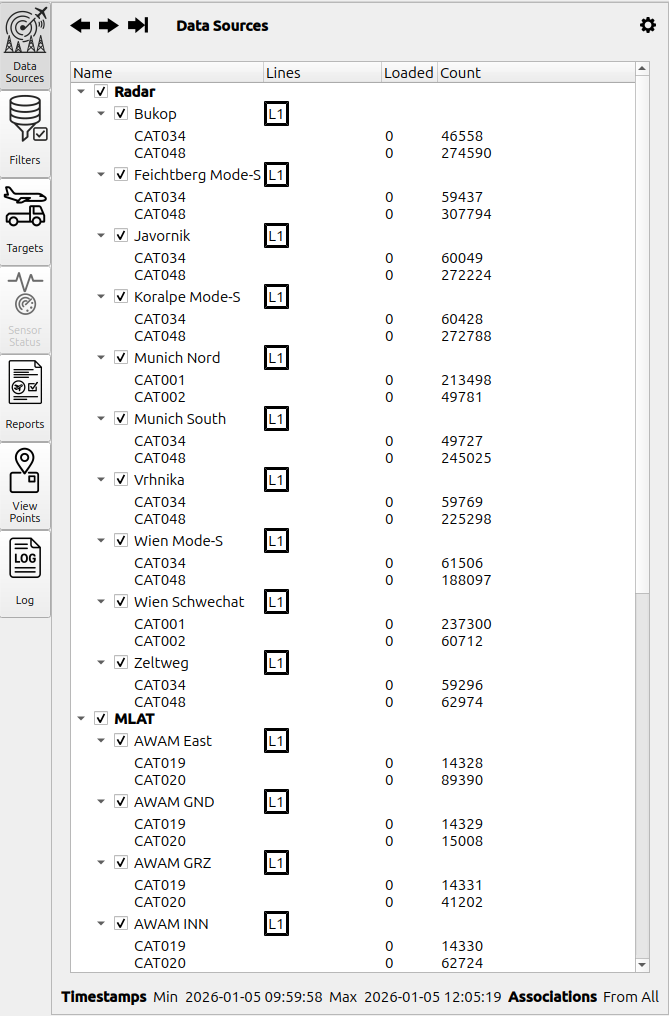
\includegraphics[width=14cm,frame]{figures/ui_data_sources.png}
  \caption{Data Sources Overview}
\end{figure}

In this Flight Deck tool, the Data Sources existing in the database are shown. 
Data sources are added to the database if data during the import process was associated with the respective Data Source (and the respective Data Source line). \\

Data Sources are grouped by DSType (Data Source Type, e.g. Radar, MLAT, ...), and can have up to 4 active lines (L1-L4). Each line for which data exists in the database is shown as a button. \\

Loading of the respective data can be changed on 3 levels:

\begin{itemize}
 \item By DSType (using checkbox)
 \item By Data Source (using checkbox)
 \item By Data Source line (using button, strong border means active)
\end{itemize}
\  \\

At the bottom, the 'Associations' label indicates if association information exists, and from which Data Source it was generated.\newline

The \includegraphics[width=0.5cm,frame]{../../data/icons/edit.png} button in the top right corner can be used to execute several actions for convenience.
Clicking the button opens the following menu.

\begin{figure}[H]
    \centering
    \includegraphics[width=4.5cm,frame]{figures/ui_data_source_configmenu.png}
  %\caption{Data Sources Overview}
\end{figure}

\paragraph{Select All DSTypes / Deselect All DSTypes}

Selects/deselects all listed Data Source types. The selection of individual Data Sources will remain as is.

\paragraph{Select Data Sources / Deselect Data Sources}

Can be used to conveniently select or deselect certain groups of Data Sources.

\begin{figure}[H]
    \centering
    \includegraphics[width=7cm,frame]{figures/ui_data_source_configmenu_select.png}
  %\caption{Data Sources Overview}
\end{figure}

The selection can either be applied to all Data Sources ('All'), or to Data Sources of a certain Data Source type. 

\paragraph{Set Line}

Can be used to conveniently select or deselect certain Data Source lines.

\begin{figure}[H]
    \centering
    \includegraphics[width=7cm,frame]{figures/ui_data_source_configmenu_lines.png}
  %\caption{Data Sources Overview}
\end{figure}

'Deselect All' will deselect all lines. 'Select L1' to 'Select L4' can be used to select a certain Data Source line for all Data Sources.

\textbf{Note} that if the selected line is not available, all available lines will be deselected.

\paragraph{Toggle Show Counts}

Toggles the display of loaded data counts below each listed Data Source. Example:

\begin{figure}[H]
    \centering
    \includegraphics[width=9cm,frame]{figures/ui_data_source_configmenu_counts.png}
  %\caption{Data Sources Overview}
\end{figure}

\subsection{Color Mode Selector}
\label{sec:color_mode_selector}

The Data Sources tool also hosts the global Color Mode selector that controls how all Views color their data. The available modes are:

\begin{itemize}
\item 'DSType': one color per DSType (Radar, MLAT, ADS-B, Tracker, RefTraj, Other)
\item 'DBContent': one color per DBContent type (CAT048, CAT062, ...)
\item 'Data Source': per-source base color
\item 'Data Source + Line': per-source base color combined with the per-line (L1-L4) variant
\end{itemize}
\ \\

The selected mode applies consistently to every open View and is persisted in the active Data Context. The colors used for each level are configured in the active Data Context (see \nameref{sec:configure_data_context}). See \nameref{sec:color_mode} for the full cross-View description.

\begin{figure}[H]
  \centering
    \fbox{\parbox{0.8\textwidth}{\vspace{1.5cm}\centering \textcolor{red}{\textbf{[FIGURE TODO: 'Data Sources' tool of the Flight Deck with the Color Mode selector expanded, showing the four mode options]}}\vspace{1.5cm}}}
  \caption{Color Mode selector}
\end{figure}

\subsection{Delete Data}
\label{sec:data_sources_delete_data}

The Data Sources tool can delete the surveillance data of one or more Data Sources from the active database. This removes the corresponding target reports from the database that belongs to the active Data Context (see \nameref{sec:configure_data_context}); the underlying recording files on disk are not touched. \\

The action can be reached from three places in the Data Sources tool: \\

\begin{itemize}
\item Top-right widget menu: 'Delete Data...' opens the dialog with no preselection
\item Right-click context menu on a DSType node: 'Delete...' opens the dialog with that DSType and all of its Data Sources preselected
\item Right-click context menu on a Data Source node (or its count subnode): 'Delete...' opens the dialog with only that Data Source preselected
\end{itemize}
\ \\

\begin{figure}[H]
  \centering
    \fbox{\parbox{0.8\textwidth}{\vspace{1.5cm}\centering \textcolor{red}{\textbf{[FIGURE TODO: top-right Data Sources tool menu with 'Delete Data...' highlighted]}}\vspace{1.5cm}}}
  \caption{Data Sources tool: Delete Data entry}
\end{figure}

\begin{figure}[H]
  \centering
    \fbox{\parbox{0.8\textwidth}{\vspace{1.5cm}\centering \textcolor{red}{\textbf{[FIGURE TODO: right-click context menu on a DSType node with 'Delete...' highlighted]}}\vspace{1.5cm}}}
  \caption{Data Sources tool: DSType-level Delete}
\end{figure}

\begin{figure}[H]
  \centering
    \fbox{\parbox{0.8\textwidth}{\vspace{1.5cm}\centering \textcolor{red}{\textbf{[FIGURE TODO: right-click context menu on a Data Source node with 'Delete...' highlighted]}}\vspace{1.5cm}}}
  \caption{Data Sources tool: per-source Delete}
\end{figure}

All three entry points open the same delete dialog, which lists the affected DBContent per Data Source and line and allows refining the selection before continuing. \\

\begin{figure}[H]
  \centering
    \fbox{\parbox{0.8\textwidth}{\vspace{1.5cm}\centering \textcolor{red}{\textbf{[FIGURE TODO: 'Delete Data' dialog with a preselection visible from a DSType-level entry point]}}\vspace{1.5cm}}}
  \caption{Delete Data dialog}
\end{figure}

After confirming the selection, a 'Confirm Delete' question dialog asks for final confirmation before the deletion is executed. \\


\includegraphics[width=0.5cm]{../../data/icons/hint.png} \textbf{Please note that the deletion removes the selected target reports from the active database permanently. The corresponding source recordings on disk are not affected; the data can be reimported.}

\begin{figure}[H]
  \centering
    \fbox{\parbox{0.8\textwidth}{\vspace{1.5cm}\centering \textcolor{red}{\textbf{[FIGURE TODO: 'Confirm Delete' question dialog shown before the deletion runs]}}\vspace{1.5cm}}}
  \caption{Delete Data confirmation}
\end{figure}
